% =====================================================================
%  Weight x KV-Cache Joint Quantization  --  Two-Stage Decomposition
%  VERTICAL (portrait) variant, target size ~ 5cm (W) x 22cm (H).
%  Top -> bottom pipeline:  (1) problem -> (2) Stage 1 -> (3) pools -> (4) Stage 2 -> cost.
%
%  COMPILE (standalone, pure TikZ):
%     pdflatex joint_search_figure_vertical.tex
%  The drawing is authored natively at ~5cm wide so fonts render at true size.
%  To force an EXACT box, wrap the tikzpicture:  \resizebox{5cm}{22cm}{ ... }
%
%  Color code:  W=blue(Wcol)  KV=orange(KVcol)  joint/ours=purple(Jcol)  naive=red(badcol)
% =====================================================================
\documentclass[border=3pt]{standalone}
\usepackage{amsmath}
\usepackage{amssymb}   % \circlearrowright
\usepackage{tikz}
\usetikzlibrary{positioning,arrows.meta,calc}

\definecolor{Wcol}{RGB}{31,119,180}
\definecolor{KVcol}{RGB}{230,126,34}
\definecolor{Jcol}{RGB}{142,68,173}
\definecolor{badcol}{RGB}{200,40,40}
\definecolor{goodcol}{RGB}{39,140,70}

% ---- compact mini Pareto-front glyph (~1.5 x 1.15) -------------------
\newcommand{\paretomini}[3]{% #1 color, #2 xlabel, #3 ylabel  @ local (0,0)
  \draw[-{Stealth[length=1.1mm]},gray!70] (0,0) -- (1.5,0)
        node[below=-1.5pt,font=\tiny,text=black]{#2};
  \draw[-{Stealth[length=1.1mm]},gray!70] (0,0) -- (0,1.15);
  \node[font=\tiny,rotate=90,anchor=south,inner sep=1pt] at (-0.04,0.55){#3};
  \draw[#1,line width=0.9pt] (0.12,1.0) .. controls (0.4,0.4) and (0.8,0.3) .. (1.4,0.22);
  \foreach \px/\py in {0.15/0.98,0.35/0.55,0.6/0.4,0.9/0.32,1.2/0.26,1.42/0.23}
     \fill[#1] (\px,\py) circle (1.05pt);
}

% ---- one horizontal shelf of 4 blocks, centered on local x=0 --------
\newcommand{\shelfrow}[6]{% #1 color, #2 title, #3..#6 labels
  \node[font=\tiny\bfseries,text=#1] at (1.425,0.52){#2};
  \foreach \k/\lab [count=\c from 0] in {0/#3,1/#4,2/#5,3/#6}
     \node[draw=#1,fill=#1!12,rounded corners=1pt,minimum width=0.72cm,
           minimum height=0.42cm,font=\tiny,inner sep=1pt] at (\c*0.95,0){\lab};
}

% ---- panel header chip, anchored inside the body top ----------------
\newcommand{\phead}[3]{% #1 color, #2 y(body-top), #3 title
  \node[fill=#1,text=white,font=\scriptsize\bfseries,minimum width=4.55cm,
        minimum height=0.5cm,anchor=north,inner sep=2pt,rounded corners=2pt]
        at (2.5,#2-0.05){#3};
}

\begin{document}
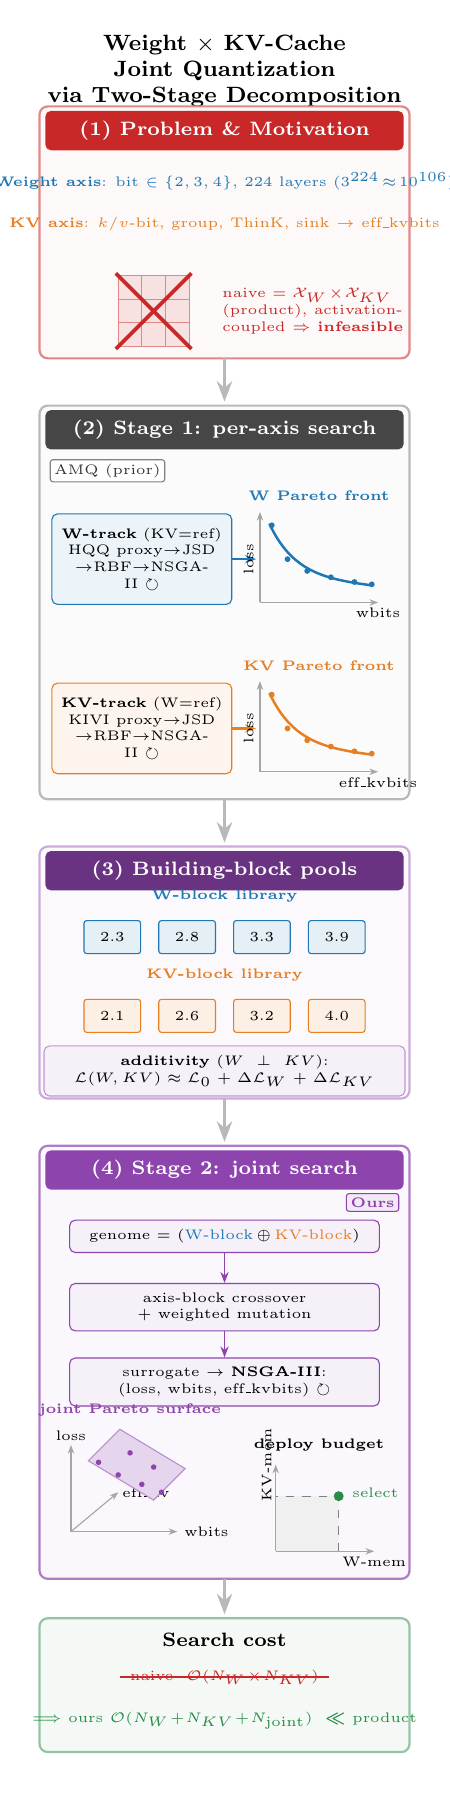
\begin{tikzpicture}[font=\sffamily]
\useasboundingbox (0,0) rectangle (5,22.1);

% ================= title =================
\node[font=\footnotesize\bfseries,align=center,text width=4.9cm] at (2.5,21.55)
   {Weight $\times$ KV-Cache Joint Quantization\\ via Two-Stage Decomposition};

% ============================================================= %
%  (1) Problem & Motivation                body 17.9 .. 21.1     %
% ============================================================= %
\draw[rounded corners=3pt,draw=badcol!55,fill=badcol!3,line width=0.8pt] (0.15,17.9) rectangle (4.85,21.1);
\phead{badcol}{21.1}{(1) Problem \& Motivation}
\node[align=center,font=\tiny,text=Wcol] at (2.5,20.15)
   {\textbf{Weight axis}: bit $\in\{2,3,4\}$, 224 layers ($3^{224}\!\approx\!10^{106}$)};
\node[align=center,font=\tiny,text=KVcol] at (2.5,19.6)
   {\textbf{KV axis}: $k/v$-bit, group, ThinK, sink $\to$ eff\_kvbits};
\begin{scope}[shift={(1.15,18.05)}]   % 3x3 product grid + cross
  \foreach \gx in {0,1,2}{\foreach \gy in {0,1,2}{
     \draw[draw=badcol!55,fill=badcol!14] (\gx*0.3,\gy*0.3) rectangle (\gx*0.3+0.3,\gy*0.3+0.3);}}
  \draw[badcol,line width=1.3pt] (-0.03,-0.03) -- (0.93,0.93);
  \draw[badcol,line width=1.3pt] (-0.03,0.93) -- (0.93,-0.03);
\end{scope}
\node[align=left,font=\tiny,text=badcol,anchor=west] at (2.35,18.5)
   {naive $=\mathcal{X}_W\!\times\!\mathcal{X}_{KV}$\\ (product), activation-\\ coupled $\Rightarrow$ \textbf{infeasible}};

% ============================================================= %
%  (2) Stage 1: decoupled per-axis search   body 12.3 .. 17.3    %
% ============================================================= %
\draw[rounded corners=3pt,draw=gray!55,fill=gray!3,line width=0.8pt] (0.15,12.3) rectangle (4.85,17.3);
\phead{gray!55!black}{17.3}{(2) Stage 1: per-axis search}
\node[draw=gray,fill=white,rounded corners=1pt,font=\tiny,text=gray!40!black,inner sep=1.5pt,
      anchor=north west] at (0.28,16.62) {AMQ (prior)};
% -- W-track --
\node[draw=Wcol,rounded corners=2pt,fill=Wcol!8,align=center,font=\tiny,
      text width=2.05cm,minimum height=1.15cm] (amqW) at (1.45,15.35)
      {\textbf{W-track} (KV$=$ref)\\ HQQ proxy$\to$JSD\\ $\to$RBF$\to$NSGA-II $\circlearrowright$};
\draw[-{Stealth[length=1.4mm]},Wcol,line width=0.8pt] (amqW.east) -- (2.9,15.35);
\begin{scope}[shift={(2.95,14.8)}] \paretomini{Wcol}{wbits}{loss} \end{scope}
\node[font=\tiny\bfseries,text=Wcol] at (3.7,16.15){W Pareto front};
% -- KV-track --
\node[draw=KVcol,rounded corners=2pt,fill=KVcol!8,align=center,font=\tiny,
      text width=2.05cm,minimum height=1.15cm] (amqK) at (1.45,13.2)
      {\textbf{KV-track} (W$=$ref)\\ KIVI proxy$\to$JSD\\ $\to$RBF$\to$NSGA-II $\circlearrowright$};
\draw[-{Stealth[length=1.4mm]},KVcol,line width=0.8pt] (amqK.east) -- (2.9,13.2);
\begin{scope}[shift={(2.95,12.65)}] \paretomini{KVcol}{eff\_kvbits}{loss} \end{scope}
\node[font=\tiny\bfseries,text=KVcol] at (3.7,14.0){KV Pareto front};

% ============================================================= %
%  (3) Building-block pools                 body 8.5 .. 11.7     %
% ============================================================= %
\draw[rounded corners=3pt,draw=Jcol!45,fill=Jcol!3,line width=0.8pt] (0.15,8.5) rectangle (4.85,11.7);
\phead{Jcol!75!black}{11.7}{(3) Building-block pools}
\begin{scope}[shift={(1.075,10.55)}] \shelfrow{Wcol}{W-block library}{2.3}{2.8}{3.3}{3.9}\end{scope}
\begin{scope}[shift={(1.075,9.55)}]  \shelfrow{KVcol}{KV-block library}{2.1}{2.6}{3.2}{4.0}\end{scope}
\node[draw=Jcol!55,fill=Jcol!8,rounded corners=2pt,align=center,font=\tiny,text width=4.35cm]
      at (2.5,8.85) {\textbf{additivity} ($W\!\perp\!KV$):\ $\mathcal{L}(W,KV)\!\approx\!\mathcal{L}_0+\Delta\mathcal{L}_W+\Delta\mathcal{L}_{KV}$};

% ============================================================= %
%  (4) Stage 2: joint combination search    body 2.4 .. 7.9      %
% ============================================================= %
\draw[rounded corners=3pt,draw=Jcol!70,fill=Jcol!4,line width=0.8pt] (0.15,2.4) rectangle (4.85,7.9);
\phead{Jcol}{7.9}{(4) Stage 2: joint search}
\node[draw=Jcol,fill=Jcol!12,rounded corners=1pt,font=\tiny\bfseries,text=Jcol,inner sep=1.5pt,
      anchor=north east] at (4.72,7.3){Ours};
\node[draw=Jcol,rounded corners=2pt,fill=Jcol!8,align=center,font=\tiny,text width=3.7cm] (gen) at (2.5,6.75)
      {genome $=$ (\textcolor{Wcol}{W-block}\,$\oplus$\,\textcolor{KVcol}{KV-block})};
\node[draw=Jcol,rounded corners=2pt,fill=Jcol!8,align=center,font=\tiny,text width=3.7cm] (ops) at (2.5,5.85)
      {axis-block crossover $+$ weighted mutation};
\node[draw=Jcol,rounded corners=2pt,fill=Jcol!8,align=center,font=\tiny,text width=3.7cm] (nsga) at (2.5,4.9)
      {surrogate $\to$ \textbf{NSGA-III}: (loss, wbits, eff\_kvbits) $\circlearrowright$};
\draw[-{Stealth[length=1.4mm]},Jcol] (gen) -- (ops);
\draw[-{Stealth[length=1.4mm]},Jcol] (ops) -- (nsga);
% outputs row: 3D joint Pareto surface  +  2D budget box
\begin{scope}[shift={(0.55,3.0)}]
  \draw[-{Stealth[length=1.1mm]},gray!70] (0,0) -- (1.35,0) node[right=-1pt,font=\tiny,text=black]{wbits};
  \draw[-{Stealth[length=1.1mm]},gray!70] (0,0) -- (0,1.1) node[above=-2pt,font=\tiny,text=black]{loss};
  \draw[-{Stealth[length=1.1mm]},gray!70] (0,0) -- (0.6,0.5) node[right=-2pt,font=\tiny,text=black]{eff\_kv};
  \fill[Jcol!22,draw=Jcol!60] (0.22,0.9) -- (1.05,0.4) -- (1.45,0.8) -- (0.62,1.3) -- cycle;
  \foreach \px/\py in {0.35/0.88,0.6/0.72,0.9/0.6,1.15/0.5,0.75/1.0,1.05/0.82}
     \fill[Jcol] (\px,\py) circle (1.0pt);
  \node[font=\tiny\bfseries,text=Jcol] at (0.75,1.55){joint Pareto surface};
\end{scope}
\begin{scope}[shift={(3.15,2.75)}]
  \draw[-{Stealth[length=1.1mm]},gray!70] (0,0) -- (1.25,0) node[below=-1.5pt,font=\tiny,text=black]{W-mem};
  \draw[-{Stealth[length=1.1mm]},gray!70] (0,0) -- (0,1.1) node[left=-2pt,font=\tiny,text=black,rotate=90,anchor=south]{KV-mem};
  \fill[gray!12] (0,0) rectangle (0.8,0.7);
  \draw[dashed,gray] (0.8,0) -- (0.8,0.7) -- (0,0.7);
  \fill[goodcol] (0.8,0.7) circle (1.8pt);
  \node[font=\tiny,text=goodcol,anchor=west] at (0.85,0.75){select};
  \node[font=\tiny\bfseries] at (0.55,1.35){deploy budget};
\end{scope}

% ============================================================= %
%  cost ribbon                              body 0.2 .. 1.9      %
% ============================================================= %
\draw[rounded corners=3pt,draw=goodcol!50,fill=goodcol!5,line width=0.8pt] (0.15,0.2) rectangle (4.85,1.9);
\node[font=\scriptsize\bfseries] at (2.5,1.62){Search cost};
\node[font=\tiny,text=badcol] (naive) at (2.5,1.15){naive\ \ $\mathcal{O}(N_W\!\times\!N_{KV})$};
\draw[badcol,line width=0.7pt] (naive.west) -- (naive.east);
\node[font=\tiny,text=goodcol,align=center] at (2.5,0.6)
   {$\Longrightarrow$\ ours\ $\mathcal{O}(N_W\!+\!N_{KV}\!+\!N_{\text{joint}})\ \boldsymbol{\ll}$ product};

% ============================================================= %
%  vertical inter-panel arrows (down the middle)                %
% ============================================================= %
\foreach \ya/\yb in {17.9/17.35, 12.3/11.75, 8.5/7.95, 2.4/1.95}
   \draw[-{Stealth[length=2.6mm]},line width=1.1pt,gray!55] (2.5,\ya) -- (2.5,\yb);

\end{tikzpicture}
\end{document}
